% !TEX TS-program = pdflatex
\documentclass[final,3p,times]{elsarticle}
\usepackage{booktabs}
\usepackage{tabularx}
\usepackage{amsmath}
\usepackage{amssymb}
\usepackage{listings}
\usepackage{placeins}
\usepackage{url}
\usepackage[hidelinks]{hyperref}
\usepackage{graphicx}
\graphicspath{{figures/}}
\setlength{\textfloatsep}{10pt plus 2pt minus 2pt}
\setlength{\dbltextfloatsep}{10pt plus 2pt minus 2pt}
\lstset{basicstyle=\ttfamily\footnotesize,breaklines=true,columns=fullflexible}
\bibliographystyle{elsarticle-num}
\journal{Computer Physics Communications}

\begin{document}
\begin{frontmatter}
\title{VARNEB: A calculator-agnostic and reproducible Python framework for variable-cell nudged elastic band calculations}

% Draft metadata: confirm author order, affiliations, and contacts before submission.
\author[a]{Xudong Zhu}
\author[a]{VARNEB contributors}
\address[a]{Affiliation and postal address to be confirmed before submission}

\begin{abstract}
Crystal phase transitions require a minimum-energy path in a space containing
both atomic and cell degrees of freedom, whereas commonly available
calculator-independent nudged elastic band (NEB) implementations are
fixed-cell. We present VARNEB, an open-source Python framework for
variable-cell NEB (VC-NEB) calculations through a common ASE-compatible
energy--force--stress contract. VARNEB represents an image by fractional
atomic coordinates and a deformation gradient, transforms atomic forces and
stress into one extended coordinate metric, and supports ordinary and
climbing-image paths, cell interpolation, endpoint mapping, restart, durable
image caching, and manager-controlled concurrent image workers. Analytic
finite-difference and fixed-cell comparisons test the coordinate and force
conventions. Two ABACUS/PBE material cases demonstrate evidence-oriented
reporting: BaTiO$_3$ tetragonal-to-cubic paths are monotonic and
image-count-independent at 5, 7, and 9 total images, while a 12-atom HfO$_2$
tetragonal-to-polar-orthorhombic path yields a 7-image climbing-image barrier
of 32.29 meV per formula unit, close to a qualified 40-image literature
reference of 32 meV per formula unit. The package does not claim a new
VC-NEB formalism; its contribution is a transparent, calculator-agnostic,
restartable implementation with explicit numerical and provenance checks.
\end{abstract}

\begin{keyword}
nudged elastic band \sep variable cell \sep crystal phase transition \sep
minimum-energy path \sep ABACUS \sep ASE \sep reproducible software
\end{keyword}
\end{frontmatter}

{\bf PROGRAM SUMMARY}
\begin{small}
\noindent {\em Program Title: VARNEB}\\
\noindent {\em CPC Library link to program files:} to be assigned under proof\\
\noindent {\em Developer's repository link:} \url{https://github.com/xdzhu/varneb}\\
\noindent {\em Licensing provisions: GNU General Public License 3.0 or later}\\
\noindent {\em Programming language: Python}\\
\noindent {\em Nature of problem:} Conventional NEB implementations commonly
assume a shared simulation cell. Solid--solid transitions may change cell
lengths, angles, and volume, and require atomic and cell forces to be treated
in a common path metric. Robust production workflows must also retain endpoint
mapping, calculator settings, scheduler resources, restart state, and
image-level evidence.\\
\noindent {\em Solution method:} VARNEB represents each image by fractional
atomic coordinates and a reference-cell deformation gradient. Cartesian forces
and stress are transformed into generalized forces before the improved tangent,
spring, and climbing-image projections are evaluated. Calculator adapters
return energy, force, and stress through ASE-compatible interfaces. A single
manager owns the path while isolated workers evaluate interior images
concurrently. JSON summaries, trajectories, audits, source-data exports, and
strict or explicitly re-audited force criteria provide reproducible reports.
\end{small}

\section{Introduction}
\label{sec:introduction}

Solid--solid phase transitions couple collective atomic motion to changes in
the lattice. This makes a fixed-cell reaction coordinate insufficient when the
minimum-energy path changes volume, shape, or shear. Variable-cell NEB was
formulated for such transitions by Qian \emph{et al.}\ \cite{Qian2013}; related
generalized solid-state NEB and finite-deformation approaches clarify the role
of cell metrics and work-conjugate stress measures
\cite{Sheppard2012,Ghasemi2019}. These methods establish that VC-NEB is not a
new algorithmic problem. The remaining software problem is to make its
conventions, calculator interface, cluster execution, recovery behaviour, and
evidence trail accessible and testable in a modern open workflow.

ASE provides a widely used calculator abstraction and fixed-cell NEB tools
\cite{Larsen2017}, but its NEB object does not optimize periodic images with
different cells. Production first-principles calculations also require more
than an optimizer loop: every image needs an isolated calculator directory,
the path controller must prevent endpoint recomputation and worker races, and
force, stress, image-count, and restart diagnostics must remain auditable.

VARNEB addresses these requirements as a pure-Python package. It treats VASP
\cite{Kresse1996a,Kresse1996b}, ABACUS \cite{Li2016}, and future calculators as
external ASE-compatible providers of energy, Cartesian forces, and stress.
The current production evidence is ABACUS/PBE. VASP is included as a
single-image adapter smoke test, not as a material-path benchmark. This
separation is important: an interface feature is not itself cross-engine
validation.

\section{From conventional NEB to VCNEB}
\label{sec:method}

\subsection{Conventional fixed-cell NEB}

For a fixed simulation cell, an image is represented only by its Cartesian
coordinate vector $R_i\in\mathbb{R}^{3N}$.  NEB finds a discretized
minimum-energy path by retaining the physical force perpendicular to the local
path tangent $\hat\tau_i$ and adding a spring force parallel to it.  With
$d_i^{\pm}=\lVert R_{i\pm1}-R_i\rVert$, the standard interior-image force is
\begin{equation}
 f_i^{\mathrm{NEB}}=
 f_i-(f_i\cdot\hat\tau_i)\hat\tau_i+
 k_i(d_i^+-d_i^-)\hat\tau_i .
 \label{eq:fixed-neb}
\end{equation}
This separation prevents the true force from sliding images down the path while
the springs control their spacing.  A climbing image replaces this expression
only after an ordinary band has formed an interior energy maximum: it reverses
the tangent component of the true force and removes the spring
\cite{Henkelman2000}.  Fixed-cell NEB is therefore recovered whenever every
image shares the same $h$ and cell degrees of freedom are inactive.

\subsection{Variable-cell generalized coordinates}

For an image with $N$ atoms, let $h$ be the row-vector cell matrix, $s_a$ the
fractional coordinate of atom $a$, and $h_0$ a reference cell. VARNEB writes
\begin{equation}
 r_a=s_a h,\qquad h=h_0F^T,
\end{equation}
where $F$ is a deformation gradient. The optimizer coordinate is
\begin{equation}
 x(Q)=\left(\operatorname{vec}(s h_0),c\operatorname{vec}(F-I)\right),
 \label{eq:coordinate}
\end{equation}
with $c$ a user-visible cell scale. Thus $c$ is a numerical metric choice, not
a material constant, and is recorded in summaries and sensitivity checks.

At hydrostatic pressure $P$, the target is $H(Q)=E(Q)+P\Omega(Q)$. For
calculator stress $\sigma$, the row-vector convention gives the cell
contribution through
\begin{equation}
 W=-\Omega(\sigma+PI),\qquad g_F=WF^{-T}.
 \label{eq:cellforce}
\end{equation}
The atomic and cell blocks are transformed into the common coordinate in
Eq.~\ref{eq:coordinate} before tangential projection.  Thus the fixed-cell
construction in Eq.~\ref{eq:fixed-neb} carries over without assigning
independent, incompatible reaction coordinates to atoms and the lattice.  For
internal image $i$, the ordinary generalized path force is
\begin{equation}
 g_i^{\mathrm{NEB}}=g_i-(g_i\cdot\tau_i)\tau_i+
 k_i(d_i^+-d_i^-)\tau_i.
 \label{eq:nebforce}
\end{equation}
The climbing-image replacement reverses the tangential component of the true
generalized force and removes the spring. CI is enabled only after an ordinary
path has a real interior enthalpy peak above both endpoints. A negative local
tangent curvature alone is not enough: a monotonic band can otherwise produce
a formal highest internal image that is not a transition state
\cite{Henkelman2000}.

Endpoint mapping and periodic translation gauge are validated before an
expensive run. The path preflight records minimum periodic atom separation,
cell deformation, segment length, and folded junctions. Summaries retain the
maximum generalized force, atom-force and stress components, reaction enthalpy,
barrier, peak identity, and CI status. An explicit post-run loose NEB re-audit
never changes the trajectory or its calculator settings.

\section{Calculator-agnostic architecture and reproducible workflow}
\label{sec:software}

The core receives no program-specific input keywords.  Its calculator contract
requires only finite energy, Cartesian forces and stress for every image;
missing stress is a hard failure because it makes the cell generalized force
undefined.  A backend adapter is responsible for units, stress convention,
static single-point semantics and a unique working directory.  In particular,
ABACUS, VASP and QE must not perform their own ionic or cell relaxation inside
an image: the manager is the sole owner of $Q_i$ updates.  This division lets
the same path algorithm operate on any ASE-compatible provider while keeping
calculator-specific pseudopotential and convergence choices visible in the
run manifest.

The ABACUS, VASP and QE factories construct one calculator directory per image;
no worker shares mutable files with another image. A controller owns image
order, endpoints, tangent construction, optimizer state, snapshots, and final
summary. A threaded executor delegates only interior calculator calls.
Endpoints are fixed and cached during a path, so a 7-total-image calculation
has five costly interior images rather than seven repeated endpoint evaluations.

The durable image cache is keyed by exact configuration plus calculator
namespace. If a batch partially fails, completed sibling evaluations remain
available and the manager emits a structured failure report. Restart selects a
complete chain snapshot; it does not regenerate an interpolation or overwrite
the original initial chain.

\begin{table*}[t]
\centering
\caption{Current VARNEB capabilities and evidence boundaries.}
\label{tab:capabilities}
\begin{tabularx}{\textwidth}{p{0.24\textwidth}X p{0.27\textwidth}}
\toprule
Capability & Delivered behaviour & Evidence boundary \\
\midrule
Extended VC-NEB coordinate & Fractional atom coordinates, deformation gradient,
force/stress transformation, pressure and cell masks & Analytic finite differences
and fixed-cell reduction tests \\
Path search & Ordinary NEB, staged CI, FIRE/BFGS/LBFGS interfaces, linear or
log-strain cell interpolation & CI requires an interior-barrier gate \\
Mode APIs & Initial-path guidance, strict subspace and projected-update modes,
release-and-refine analytic example & A real-material release diagnostic is
archived at a loose $0.10$ eV/\AA{} snapshot; strict $0.05$ eV/\AA{} release
comparison remains incomplete \\
Execution & Isolated image directories, manager/worker ownership, bounded retry,
snapshots, resume and durable cache & Scheduler resources remain user-reviewed \\
Calculators & ABACUS, VASP and QE ASE-facing factories & ABACUS has material paths;
VASP has a single-image smoke test and QE has a static no-DFT preflight only \\
Reporting & JSON summary, trajectory, audit, image comparison, structural metrics,
source-data and editable figure export & Results remain calculator and
boundary-condition specific \\
\bottomrule
\end{tabularx}
\end{table*}

A production run prepares element-preserving endpoint structures with identical
atom count, independently relaxes and audits them, preflights a mapped and
translation-aligned initial path, runs ordinary VC-NEB with cached endpoints,
compares image counts, and only then enables CI. The command-line driver
exposes image count, cell interpolation, mapping, force threshold, image
workers, and resume state rather than choosing them implicitly.

\begin{lstlisting}[caption={Illustrative ABACUS production invocation.},label={lst:abacus}]
python examples/run_vcneb_abacus.py \
  --initial relaxed_T/CONTCAR --final relaxed_PO/CONTCAR \
  --n-images 7 --fmax 0.10 --optimizer FIRE --maxstep 0.003 \
  --cell-interpolation log_strain --mapping auto --align-translation \
  --image-workers 5 --image-retries 1 \
  --ecutwfc 100 --kpts 2 2 2 --scf-thr 1e-8
\end{lstlisting}

\section{Validation and material examples}
\label{sec:results}

An analytic coupled atomic--cell multiwell potential supplies a known minimum,
saddle, and 0.25 eV barrier. Finite-difference tests cover atomic forces, cell
forces, nonzero pressure, and nonorthogonal cells. A fixed-cell comparison with
ASE NEB/CINEB gives a barrier difference of $9.33\times10^{-6}$ eV under the
matched test convention. These tests establish implementation consistency, not
first-principles predictive accuracy.

\subsection{BaTiO$_3$ tetragonal to cubic path}

BaTiO$_3$ is a compact direct perovskite case. ABACUS/PBE calculations use
100 Ry and full 10-au DZP Ba/Ti/O orbitals, a $4\times4\times4$ k mesh, and
independently relaxed fixed endpoints. Ordinary 5-, 7-, and 9-total-image paths
converge below $0.02$ eV/\AA{} maximum generalized force and are all monotonic.
Their reaction enthalpy is $0.0871289$ eV per formula unit; there is no interior
barrier, so CI is correctly withheld. A tighter $6\times6\times6$ and $10^{-9}$
SCF comparison preserves the path topology but shifts the absolute endpoint
difference by about 15 meV.

The result corresponds to $2.01$ kcal mol$^{-1}$ and is close in energy scale
to a reported $2.1$ kcal mol$^{-1}$ restrained PBEsol NEB result
\cite{BTOReaxFF2019}. This is not a strict algorithm benchmark: the literature
calculation uses different exchange-correlation treatment and local restraints,
whereas the present result is an unconstrained variable-cell path.

To separate a path-coordinate description from a phonon claim, we also evaluated
the cubic endpoint with a $1\times1\times1$ finite-displacement calculation
($\delta=0.01$ \AA{}, six signed displacements) and assembled the $\Gamma$-point
force constants and direct $\Gamma$ eigenvectors with Phonopy \cite{Togo2015}.
The ABACUS--Phonopy force-constant convention,
$\mathrm{eV}/(\AA\,\mathrm{au})$, is retained explicitly in the provenance
of the direct Phonopy $q=0$ calculation. The spectrum contains a triply degenerate unstable
subspace at $-298.956$ cm$^{-1}$. After applying the
recorded O-atom permutation and endpoint translation gauge, then removing each
image's mass-weighted rigid translation, the seven-image T-to-C atomic path has
a maximum soft-subspace coordinate norm of $1.2043\sqrt{\mathrm{amu}}$\AA{} and
a maximum segment-tangent overlap of 0.9974 with that subspace. The complete-mode
reconstruction residual is below $5.9\times10^{-16}\sqrt{\mathrm{amu}}$\AA{}.
The $175.809$ cm$^{-1}$ stable triplet also participates (maximum coordinate norm
$0.2863\sqrt{\mathrm{amu}}$\AA{}), so this is a subspace-resolved mechanism
analysis rather than an assertion that one arbitrarily phased eigenvector alone
defines the path. Homogeneous cell strain remains a separate VC-NEB coordinate,
not a phonon amplitude.

\begin{figure*}[t]
\centering
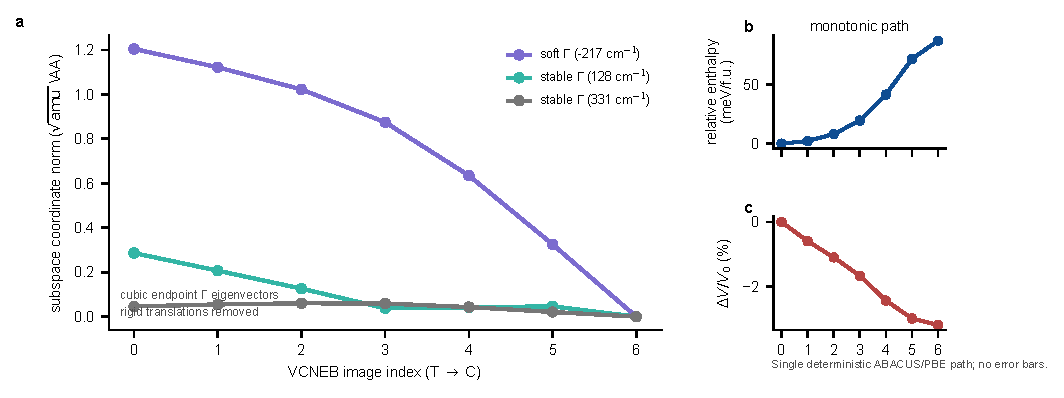
\includegraphics[width=\textwidth]{bto_gamma_mode_path.pdf}
\caption{BTO T-to-C path resolved in cubic-endpoint $\Gamma$ subspaces. (a)
Mass-weighted coordinate norms after applying the recorded atom permutation and
endpoint gauge translation, then removing each image's rigid translation. The
threefold unstable subspace (purple) dominates the atomic path; stable triplets
are retained to show the residual multimode component. (b) The same seven-image
ABACUS/PBE path has no interior energy maximum. (c) Homogeneous volume evolution
is reported separately from the atomic phonon coordinates. This is one
deterministic first-principles path, so no statistical error bars are implied.
Editable source data accompany the manuscript.}
\label{fig:bto-gamma-mode}
\end{figure*}

\subsection{HfO$_2$ tetragonal to polar orthorhombic path}

The HfO$_2$ case uses an explicitly mapped 12-atom Hf$_4$O$_8$ endpoint pair:
a $\sqrt{2}\times\sqrt{2}\times1$ tetragonal supercell and a
conventional-compatible polar orthorhombic cell. ABACUS/PBE calculations use
100 Ry, full 10-au DZP Hf/O orbitals, a $2\times2\times2$ k mesh, and
independently converged endpoints. Ordinary log-strain 7- and 9-total-image
paths give barriers of 0.1567509 and 0.1562092 eV per 12-atom cell,
respectively, a spread of 0.0005417 eV. The 7-image linear-cell control is
0.1596772 eV. These controls are reported separately: the linear-cell path
tests interpolation sensitivity rather than image-count convergence.

The staged 7-image CI refinement gives 0.1291722 eV per 12-atom cell, or
32.29 meV per HfO$_2$ formula unit, at a final maximum generalized force of
0.02955 eV/\AA{}. Liu and Hanrahan reported 32 meV per formula unit for a
40-image LDA/QE/USPEX VC-NEB calculation \cite{Liu2019}. The agreement is
encouraging but deliberately qualified by functional, pseudopotential,
implementation, image-count, mapping, and force-norm differences.

A separate real-material release diagnostic starts from a strict-subspace
chain and then releases all degrees of freedom.  Its full-space force reached
0.097528 eV/\AA{} at step 275 but rebounded to 0.108376 eV/\AA{} during 25
additional observed steps.  We archive the step-275 path only under the
conventional loose 0.10 eV/\AA{} ordinary-NEB convention; it is excluded from
the strict ordinary/CI barrier comparison and literature discussion.

\begin{figure*}[t]
\centering

\includegraphics[width=\textwidth]{vcneb_material_validation.pdf}
\caption{Material validation and qualified literature comparison. (a) ABACUS/PBE
BaTiO$_3$ T-to-C paths at 5, 7, and 9 total images are monotonic; the cubic
endpoint, not an internal image, is the maximum. (b) HfO$_2$ T-to-PO ordinary
log-strain paths, a linear-cell control, and a staged CI refinement. The open
circle marks the climbing image and the dotted line denotes the external
literature CI-VCNEB barrier. (c) HfO$_2$ barriers per formula unit. The
literature bar is not a statistical replicate. (d) Relative volume evolution
demonstrates the variable-cell degree of freedom. Source data accompany this
figure in the software archive.}
\label{fig:materials}
\end{figure*}

\FloatBarrier
\section{Scope, limitations, and outlook}
\label{sec:limits}

VARNEB currently implements the documented hydrostatic enthalpy convention.
General-stress G-SSNEB and finite-deformation paths require explicit
work-conjugate stress measures and are not silently inferred from the present
interface. A converged CI path is also not a vibrational first-order-saddle
proof; targeted finite-difference mode analysis remains necessary where that
designation is required.

The material cases demonstrate one ABACUS/PBE family, not universal accuracy.
HfO$_2$ remains sensitive to mapping, supercell size, mechanical boundary
conditions, and possible intermediate mechanisms. The BTO case is deliberately
barrierless and therefore validates the CI gate rather than a saddle search.
Future work will add a production VASP path, cross-implementation comparisons,
strict $0.05$ eV/\AA{} real-material release-and-refine comparisons, and
systematic supercell and stress-measure benchmarks.

\section{Conclusions}

VARNEB provides a transparent Python implementation of variable-cell NEB with
explicit extended-coordinate, force, calculator, execution, and reporting
contracts. Analytic and fixed-cell tests validate the core mechanics, while
ABACUS/PBE BTO and HfO$_2$ cases demonstrate image-count, interpolation,
climbing-image, restart, and provenance practices. The software contribution
is not a claim of a new VC-NEB theory; it is an open and evidence-oriented
framework that makes calculator-independent variable-cell path calculations
more reproducible and easier to audit.

\section*{Data availability}

The source code, examples, tests, manuscript source, and compact source-data
tables are available at \url{https://github.com/xdzhu/varneb}. Full
first-principles output directories are retained with the project calculation
archive. The files used to generate Fig.~\ref{fig:materials} are completed
path summaries and the committed CSV tables in the software archive.

\section*{CRediT authorship contribution statement}
Draft placeholder: confirm roles and author order before submission.

\section*{Declaration of competing interest}
The authors declare no competing financial interests. Confirm this statement
with all authors before submission.

\section*{Acknowledgements}
Draft placeholder: add funding, computing allocations, and institutional
acknowledgements before submission.

\bibliography{varneb}
\end{document}
